\begin{titlepage}
  \begin{center}

  {\Huge SIPO}

  \vspace{25mm}

  
\includegraphics[width=0.90\textwidth,height=\textheight,keepaspectratio]{img/AFRL.png}

  \vspace{25mm}

  \today

  \vspace{15mm}

  {\Large Jay Convertino}

  \end{center}
\end{titlepage}

\tableofcontents

\newpage

\section{Usage}

\subsection{Introduction}

\par
This core converts the serial input data to parallel output data. This is done on a positive clock edge in relation to a active high enable.
The enable sets the rate data is sampled. This core is useful for
any serial to parallel operation such as UARTS, SPI, i2c, 1553, etc. This is a fusesoc 2.X compatible core and its VLNV is
AFRL:simple:sipo:X.X.X.

\subsection{Dependencies}

\par
The following are the dependencies of the cores.

\begin{itemize}
  \item fusesoc 2.X
  \item iverilog (simulation)
  \item cocotb (simulation)
\end{itemize}

\subsubsection{fusesoc\_info Depenecies}
\begin{itemize}
\end{itemize}


\subsection{In a Project}
\par
This core is made to be used on the same clock domain as the input parallel data. The serial input rate is set by the enable.
The enable should only be pulsed for one clock cycle. If the clock is the rate the enable should be tied high. Load has to be
used to get the output data and reset the input count. The data count provers other cores a bit count to know what bit currently being
input to the core. On load data is cleared from the input register and the count is reset to 0. Once enable is toggled the count
will increment and indicates how many bits of the word are contained in the register. The register is full once the max number
of bits is reached on the counter output.
\begin{enumerate}
  \item Set ena to 1 at rising clock edge for one clock cycle
  \item Continue till the counter hits the number of bits needed.
  \item Read the parallel data output to capture data.
  \item Assert load to 1 to restart counter and clear parallel register.
\end{enumerate}

Adding the core to a fusesoc project, outside of adding the verilog module to your code, requires it is added as dependency.
Example:
\begin{lstlisting}[language=bash]
  dep:
    depend:
      - ">=AFRL:simple:sipo:1.0.0"
\end{lstlisting}

Module instantiation:
\begin{lstlisting}[language=Verilog]
    sipo #(
      .BUS_WIDTH(4)
    ) inst_sipo (
      .clk(clk),
      .rstn(rstn),
      .ena(ena),
      .load(load),
      .pdata(pdata),
      .sdata(sdata),
      .dcount(dcount)
    );
\end{lstlisting}

\section{Architecture}
\par
This core is made to interface for serial to parallel data. On each enable pulse on a positive clock edge the input serial
line will be sampled. The counter starts at 0 and the shift is complete once it hits BUS\_WIDTH * 8. For a 32 bit word you will
need 32 enable pulses. These will correspond to counter output 0 to 31. 32 will signal the shift is done and the parallel output
data is valid. Once it is valid data can be read and load asserted. Load will reset the core and clear it for the next shift operation.
All data is shifted in MSb to LSb. Meaning Bit 31 is input first and 0 is last.
The only module is the sipo module. It is listed below.

\begin{itemize}
  \item \textbf{sipo} Convert serial data to parallel by shifting in data on each enable pulse on a rising clock. (see core for documentation).
\end{itemize}

Please see \ref{Module Documentation} for more information.

\subsection{Waveform}
Below is a waveform in a typical application of the core. This shows the count up and how the enable is pulsed to increment it.

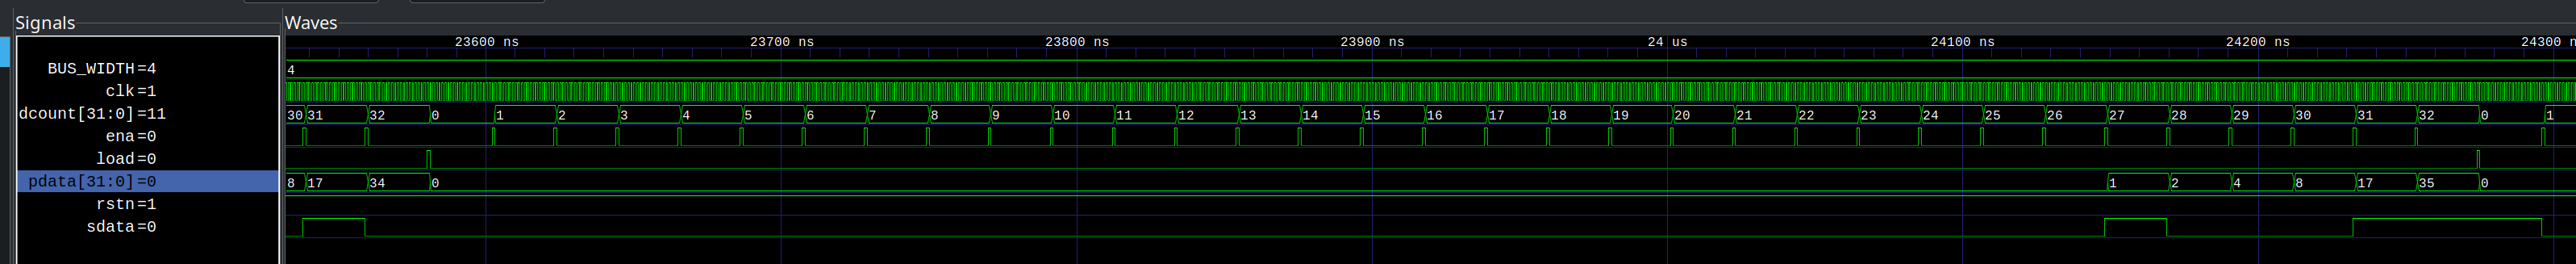
\includegraphics[width=\textwidth]{img/diagrams/waveform.png}

\section{Building}

\par
The SIPO core is written in Verilog 2001. They should synthesize in any modern FPGA software. The core comes as a fusesoc packaged core and can be included in any other core as a dependency. Be sure you have meet the dependencies listed in the previous section.

\subsection{fusesoc}
\par
Fusesoc is a system for building FPGA software without relying on the internal project management of the tool. Avoiding vendor lock in to Vivado or Quartus.
These cores, when included in a project, can be easily integrated into targets created based upon the end developer needs. The core by itself is not a part of
a system and should be integrated into a fusesoc based system. Simulations are setup to use fusesoc and are a part of its targets.

\subsection{Source Files}

\subsubsection{fusesoc\_info File List}
\begin{itemize}
\item src
	\begin{itemize}
	\item src/sipo.v
	\end{itemize}
\item tb
	\begin{itemize}
	\item tb/tb\_sipo.v
	\end{itemize}
\item tb\_cocotb
	\begin{itemize}
	\item {'tb/tb\_cocotb.py': {'file\_type': 'user', 'copyto': '.'}}
	\item {'tb/tb\_cocotb.v': {'file\_type': 'verilogSource'}}
	\end{itemize}
\end{itemize}


\subsection{Targets}

\subsubsection{fusesoc\_info Targets}
\begin{itemize}
\item default
	\begin{itemize}
	\item[$\space$] Info: Default for IP intergration.
	\end{itemize}
\item lint
	\begin{itemize}
	\item[$\space$] Info: Lint with Verible
	\end{itemize}
\item sim
	\begin{itemize}
	\item[$\space$] Info: Base simulation using icarus as default.
	\end{itemize}
\item sim\_cocotb
	\begin{itemize}
	\item[$\space$] Info: Cocotb unit tests
	\end{itemize}
\end{itemize}


\subsection{Directory Guide}

\par
Below highlights important folders from the root of the directory.

\begin{enumerate}
  \item \textbf{docs} Contains all documentation related to this project.
    \begin{itemize}
      \item \textbf{manual} Contains user manual and github page that are generated from the latex sources.
    \end{itemize}
  \item \textbf{src} Contains source files for the core
  \item \textbf{tb} Contains test bench files for iverilog and cocotb
    \begin{itemize}
      \item \textbf{cocotb} testbench files
    \end{itemize}
\end{enumerate}

\newpage

\section{Simulation}
\par
There are a few different simulations that can be run for this core. The backend used for testing is iverilog for verilog or cocotb simulations. Usually GTKWave is used to view the fst waveform output. Cocotb are the unit tests that attempt to give a pass/fail verification to the core operation.

\subsection{iverilog}
\par
iverilog is used for simple test benches for quick visual verification of the core. This will autofinish after it has
run up to a certain number of words have been output.

\subsection{cocotb}
\par
This method allows for quick writing of test benches that actually assert and check the state of the core.
These tests are much more conclusive since it will run all test vectors and generate a report if they
pass or fail. All tests generate to a single fst wave file. The method of launching the tests is to use
fusesoc. These have not been written to use the python runner method or makefiles.
To use the cocotb tests you must install the following python libraries.
\begin{lstlisting}[language=bash]
  $ pip install cocotb
\end{lstlisting}

The targets available are listed below.
\begin{itemize}
  \item \textbf{sim\_cocotb} Standard simulation PISO conversion using cocotb.
\end{itemize}

The targets above can be run with various parameters.
\begin{lstlisting}[language=bash]
  $ fusesoc run --target sim_cocotb AFRL:simple:sipo:1.0.0
\end{lstlisting}

\newpage

\section{Module Documentation} \label{Module Documentation}

\par

\begin{itemize}
\item \textbf{sipo} SIPO converter\\
\item \textbf{tb\_sipo-v} Verilog test bench\\
\item \textbf{tb\_cocotb-py} Cocotb python test routines\\
\item \textbf{tb\_cocotb-v} Cocotb verilog test bench\\
\end{itemize}
The next sections document the module in detail.

